\section{EVALUATION}
\uline{\textbf{Simulations}}: Our algorithm was implemented in MATLAB. Three case studies of path planning are considered for validation: same location and different orientation between initial configuration and goal configuration, long distance between two configuration, and bi-direction path finding.\\

\noindent\uline{\textbf{Cube solid}}:
Writing about cube solid properties\\

\noindent\uline{Case study 1}: Dennis also went his own way and divided the sides of the triangles into equal-angles (as measured from the center of the geodesic), instead of equal-length pieces. This technique is slightly more effective at evenly distributing the triangles across the surface of the sphere. For example, compare an octahedron subdivided with frequency 20, using the linear technique (as outlined by the quiz) versus the angular technique Dennis used in this picture. Note how the linear technique has the triangles piling up along the edges of the original face of the octahedron, where the radial technique does a better job of spacing them out.
\begin{center}
\begin{figure}[h]
\subfigure[The initial configuration is the same position but different orientation with goal configuration]{
	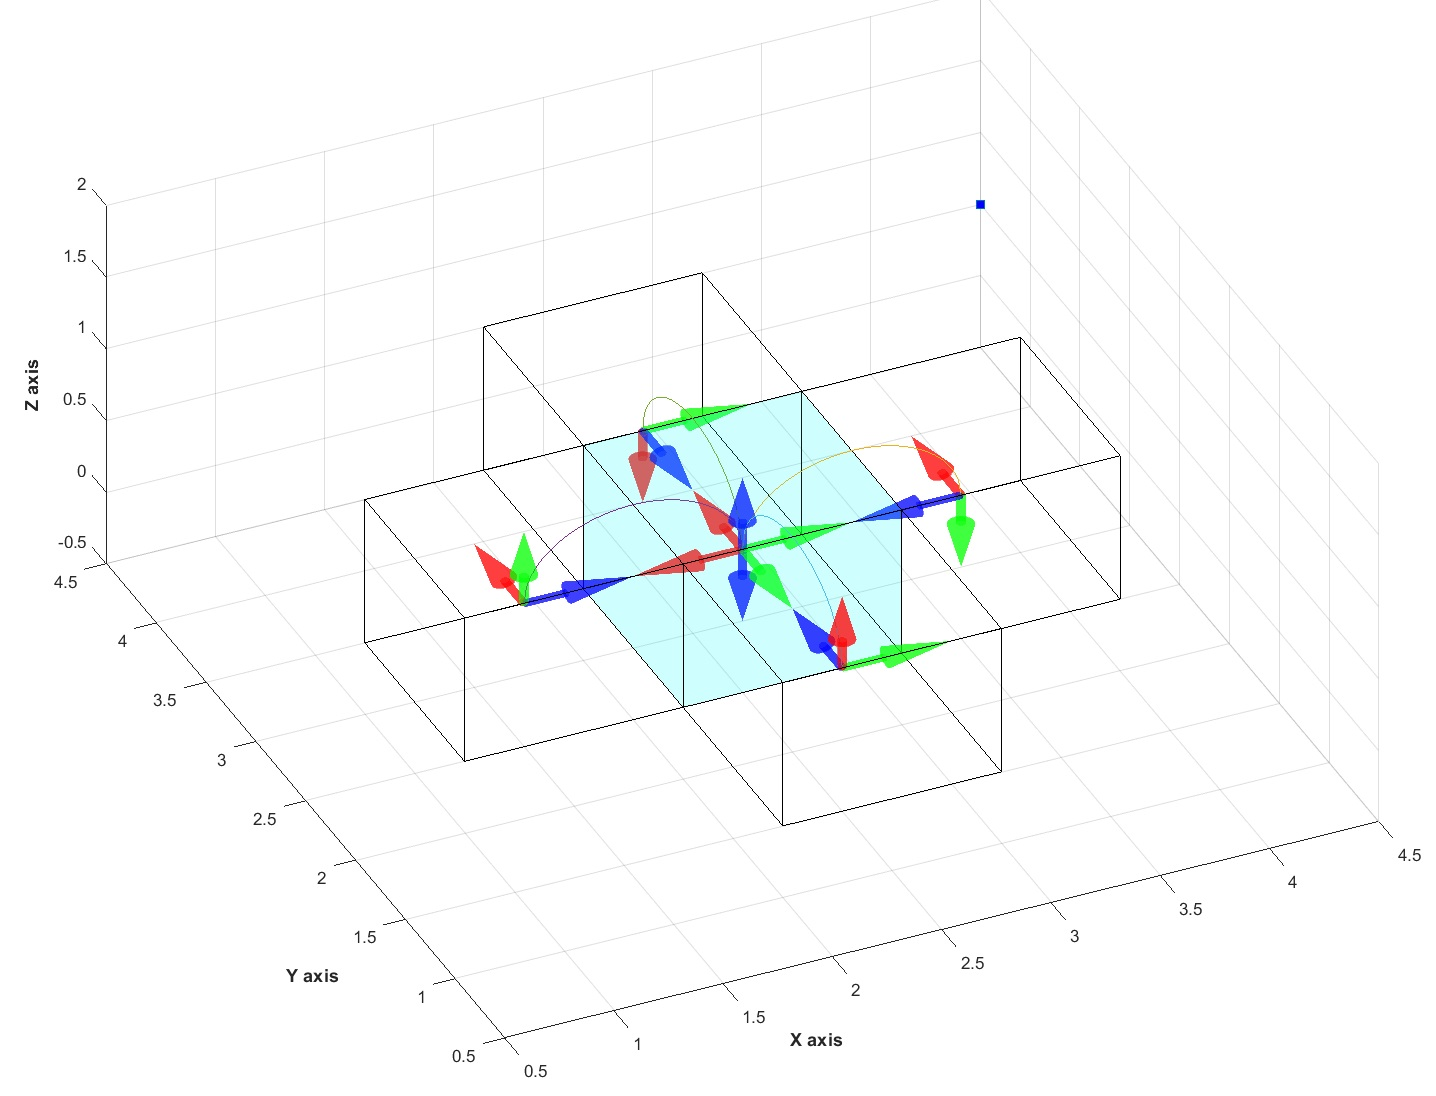
\includegraphics[width=0.5\textwidth]{image/cube11.jpg}
	\label{fig:Cube1Case1}
	}
\hfill
\subfigure[First four paths of the cube rolling]{
	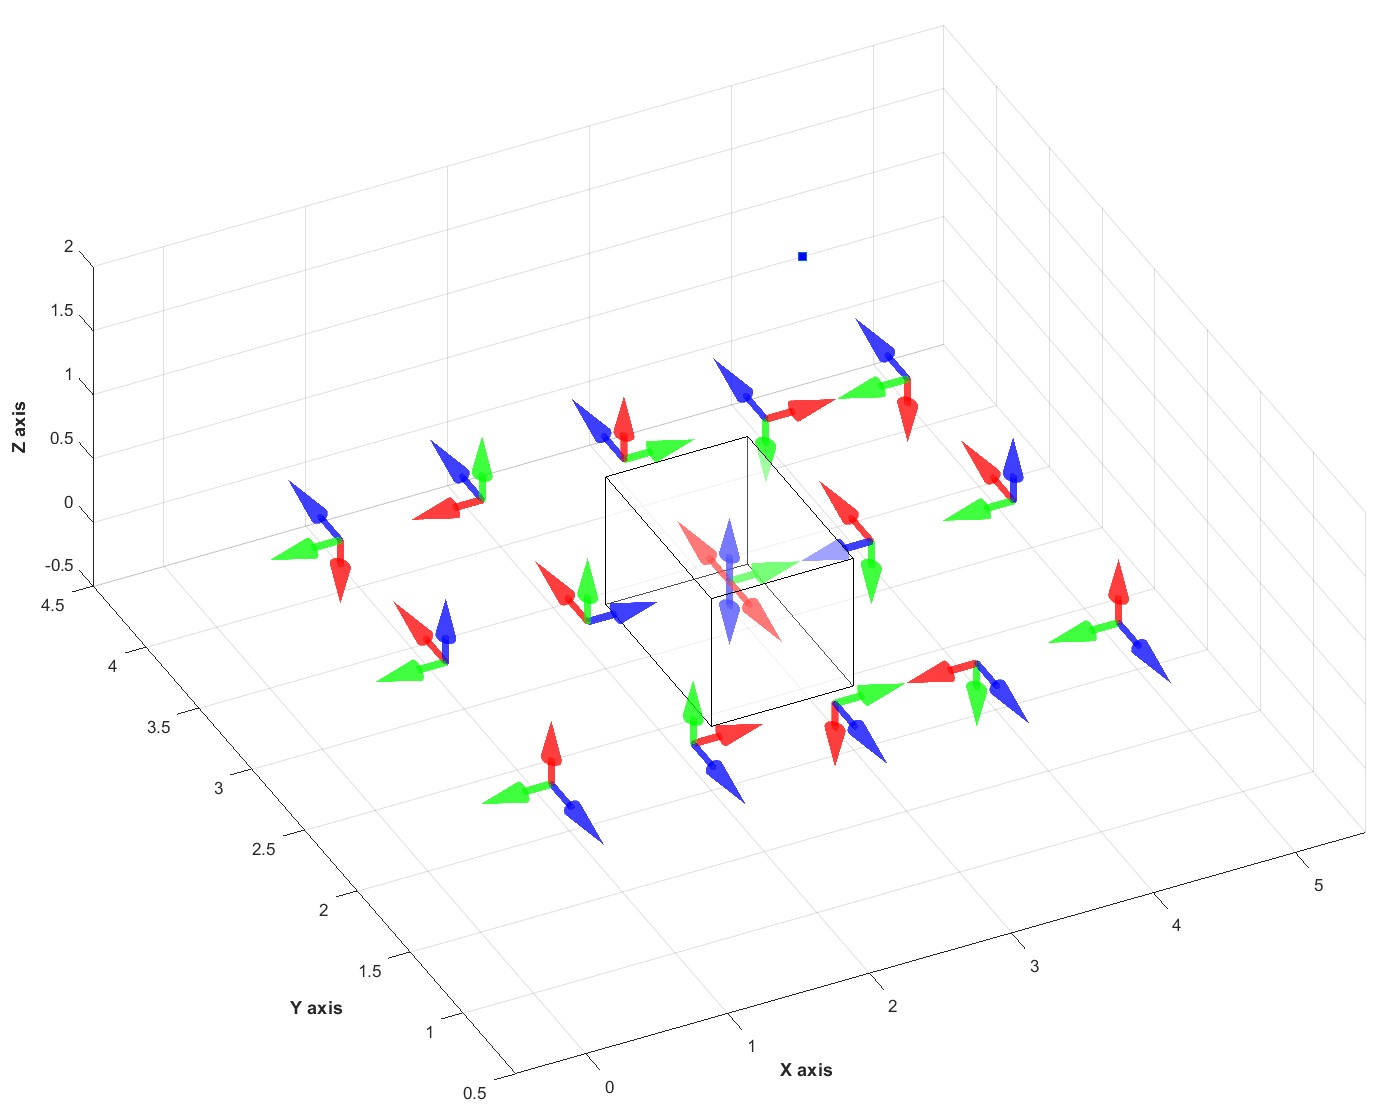
\includegraphics[width=0.5\textwidth]{image/cubePath4Dirs.jpg}
%    \includegraphics[page=2,width=.5\textwidth]{image/test2.pdf}	
	\label{fig:Cube2Case1}
	}
\caption{Blah Blah}
\end{figure}
\end{center}

\noindent\uline{Case study 2}: Long distance between two configuration:
Dennis also went his own way and divided the sides of the triangles into equal-angles (as measured from the center of the geodesic), instead of equal-length pieces. This technique is slightly more effective at evenly distributing the triangles across the surface of the sphere. For example, compare an octahedron subdivided with frequency 20, using the linear technique (as outlined by the quiz) versus the angular technique Dennis used in this picture. Note how the linear technique has the triangles piling up along the edges of the original face of the octahedron, where the radial technique does a better job of spacing them out.
%\begin{figure}[h]
%	\centering
%		\begin{subfigure}[t]
%			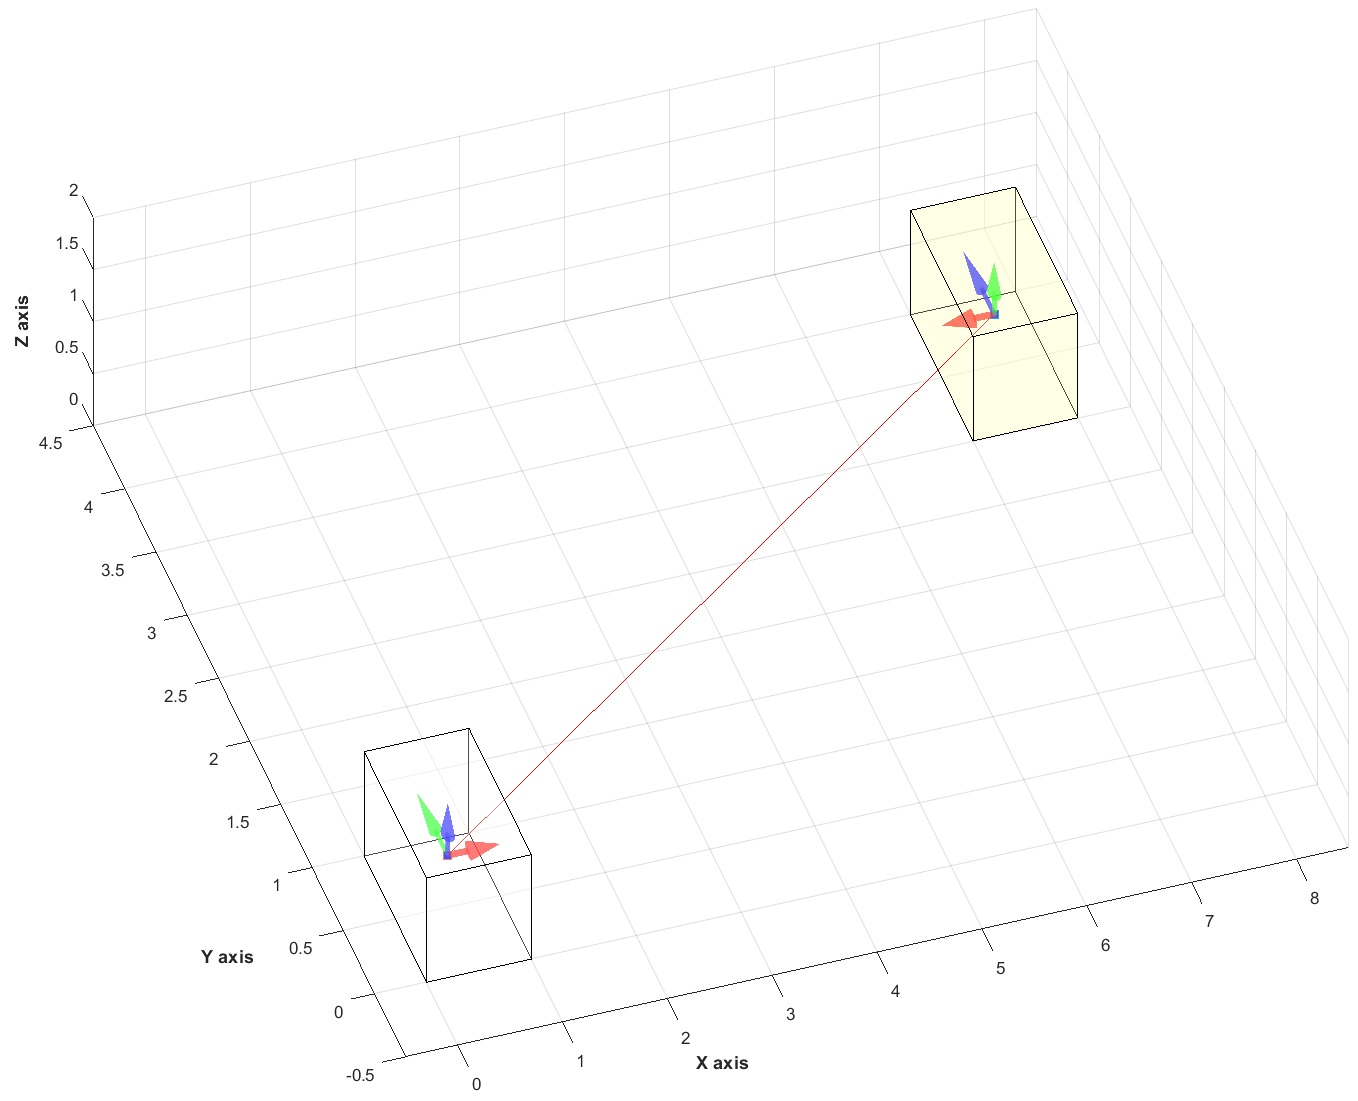
\includegraphics[width=0.5\textwidth]{image/cubePathCase2Initial.jpg}
%			\subcaption{Long distance between two configurations}
%			\label{fig:Cube1Case2}
%		\end{subfigure}
%%\hfill
%		\begin{subfigure}[t]
%			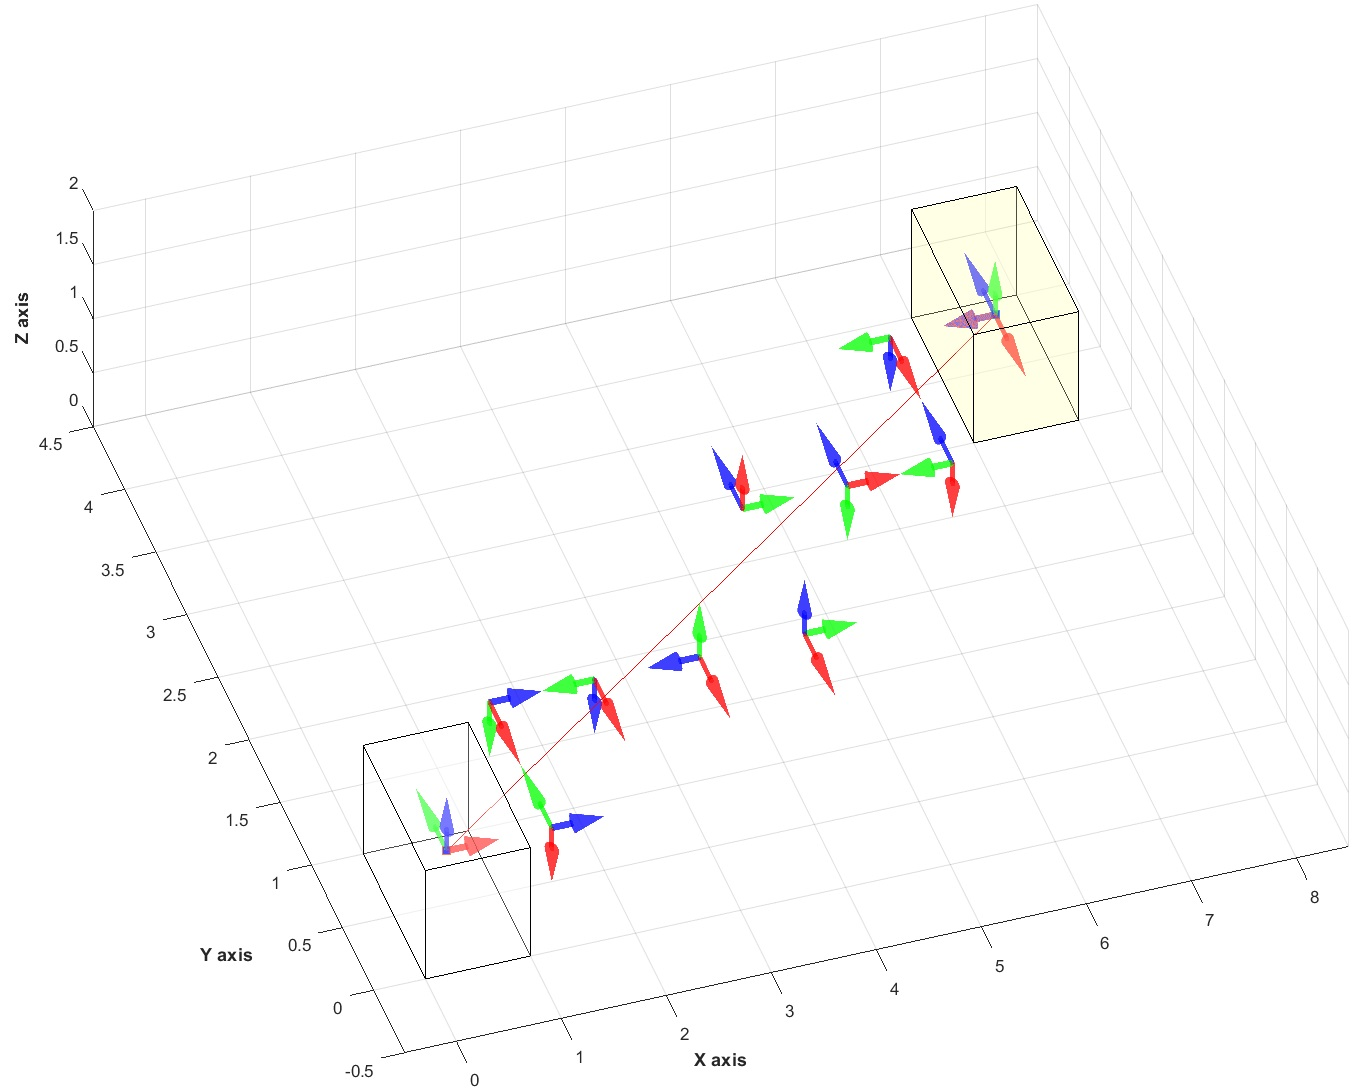
\includegraphics[width=0.5\textwidth]{image/cubePathCase2DirecRolling.jpg}
%			\subcaption{Directly rolling from initial configuration to goal configuration}
%			\label{fig:Cube2Case2}
%		\end{subfigure}
%\end{figure}
\begin{center}
\begin{figure}[h]
\subfigure[Long distance between two configurations]{
	\includegraphics[width=0.5\textwidth]{image/cubeCase2Initial.jpg}
	\label{fig:Cube1Case2}
	}
\hfill
\subfigure[Directly rolling from initial configuration to goal configuration]{
	\includegraphics[width=0.5\textwidth]{image/cubeCase2DirecRolling.jpg}
	\label{fig:Cube2Case2}
	}
\caption{Blah Blah 2}
\end{figure}
\end{center}
%%
%%
%%
\begin{center}
\begin{figure}[h]
\subfigure[Path1]{
	\includegraphics[width=0.5\textwidth]{image/cubeCase2Path1.jpg}
	\label{fig:Cube3Case2}
	}
\hfill
\subfigure[Path2]{
	\includegraphics[width=0.5\textwidth]{image/cubeCase2Path2.jpg}
	\label{fig:Cube4Case2}
	}
\caption{Blah Blah 3}
\end{figure}
\end{center}
%%
%%
%%

\noindent\uline{Case study 3}: Bi-direction path finding.\\
%%
%%
%%

\noindent\uline{Case study 4}: Cube path planning with obstacle avoiding.\\
%%
%%
%%

\noindent\uline{\textbf{Tetrahedron solid}}:
Writing about cube solid properties\\

\noindent\uline{Case study 1}:
Dennis also went his own way and divided the sides of the triangles into equal-angles (as measured from the center of the geodesic), instead of equal-length pieces. This technique is slightly more effective at evenly distributing the triangles across the surface of the sphere. For example, compare an octahedron subdivided with frequency 20, using the linear technique (as outlined by the quiz) versus the angular technique Dennis used in this picture. Note how the linear technique has the triangles piling up along the edges of the original face of the octahedron, where the radial technique does a better job of spacing them out.\\

\begin{center}
\begin{figure}[h]
\subfigure[The initial configuration is the same position but different orientation with goal configuration]{
	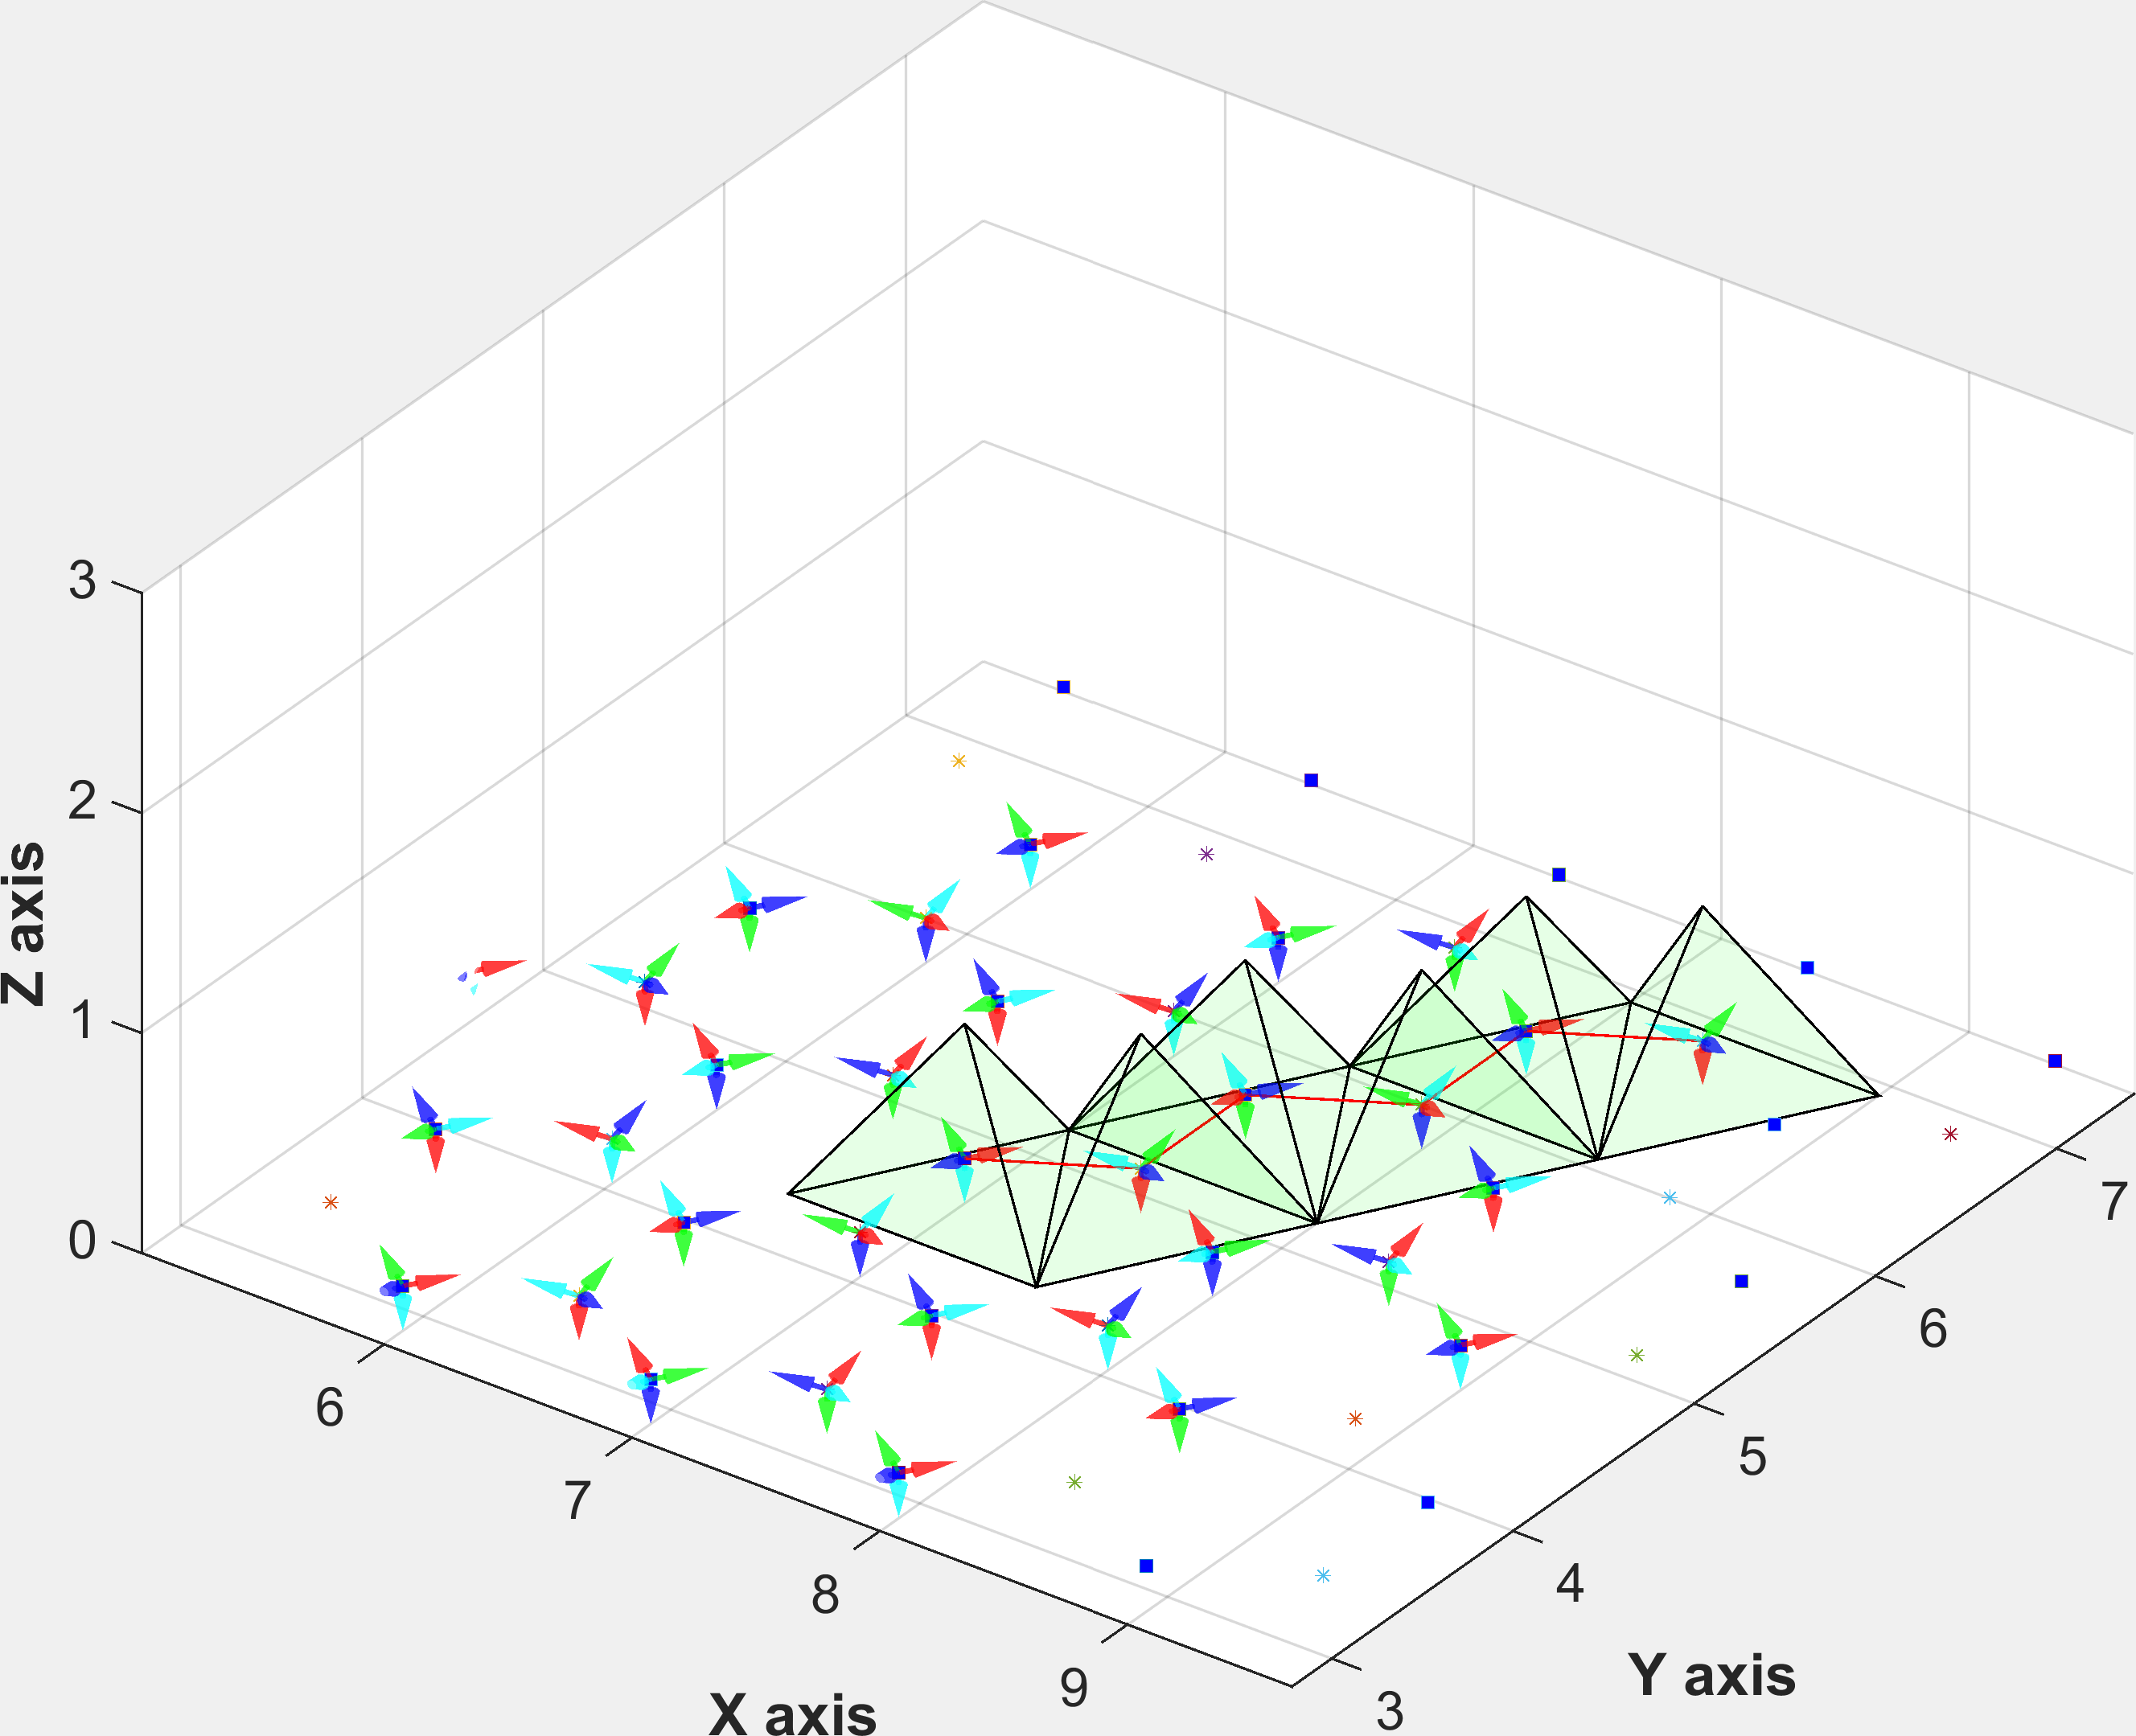
\includegraphics[width=0.5\textwidth]{image/Tetra1.png}
	\label{fig:Tetra1Case1}
	}
\hfill
\subfigure[First four paths of the cube rolling]{
	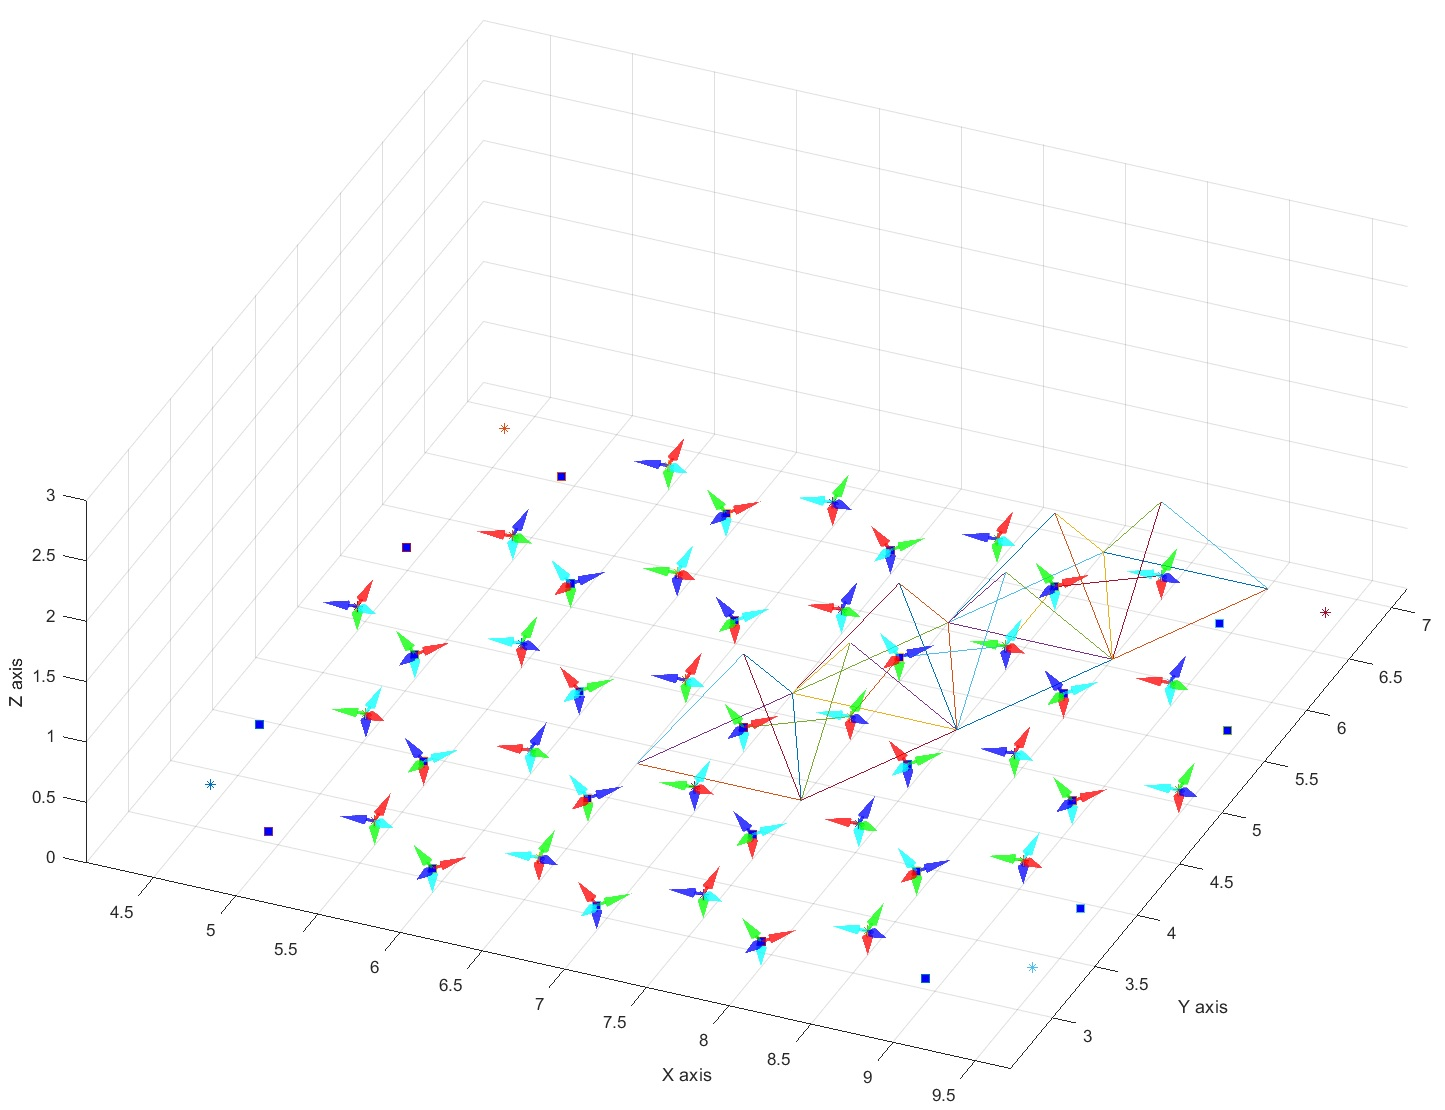
\includegraphics[width=0.5\textwidth]{image/TetraPath1.jpg}
	\label{fig:Tetra2Case1}
	}
\caption{Blah Blah Tetra}
\end{figure}
\end{center}

\noindent\uline{Case study 2}: Long distance between two configuration:
Dennis also went his own way and divided the sides of the triangles into equal-angles (as measured from the center of the geodesic), instead of equal-length pieces. This technique is slightly more effective at evenly distributing the triangles across the surface of the sphere. For example, compare an octahedron subdivided with frequency 20, using the linear technique (as outlined by the quiz) versus the angular technique Dennis used in this picture. Note how the linear technique has the triangles piling up along the edges of the original face of the octahedron, where the radial technique does a better job of spacing them out.\\

\begin{center}
\begin{figure}[h]
\subfigure[The initial configuration is the same position but different orientation with goal configuration]{
	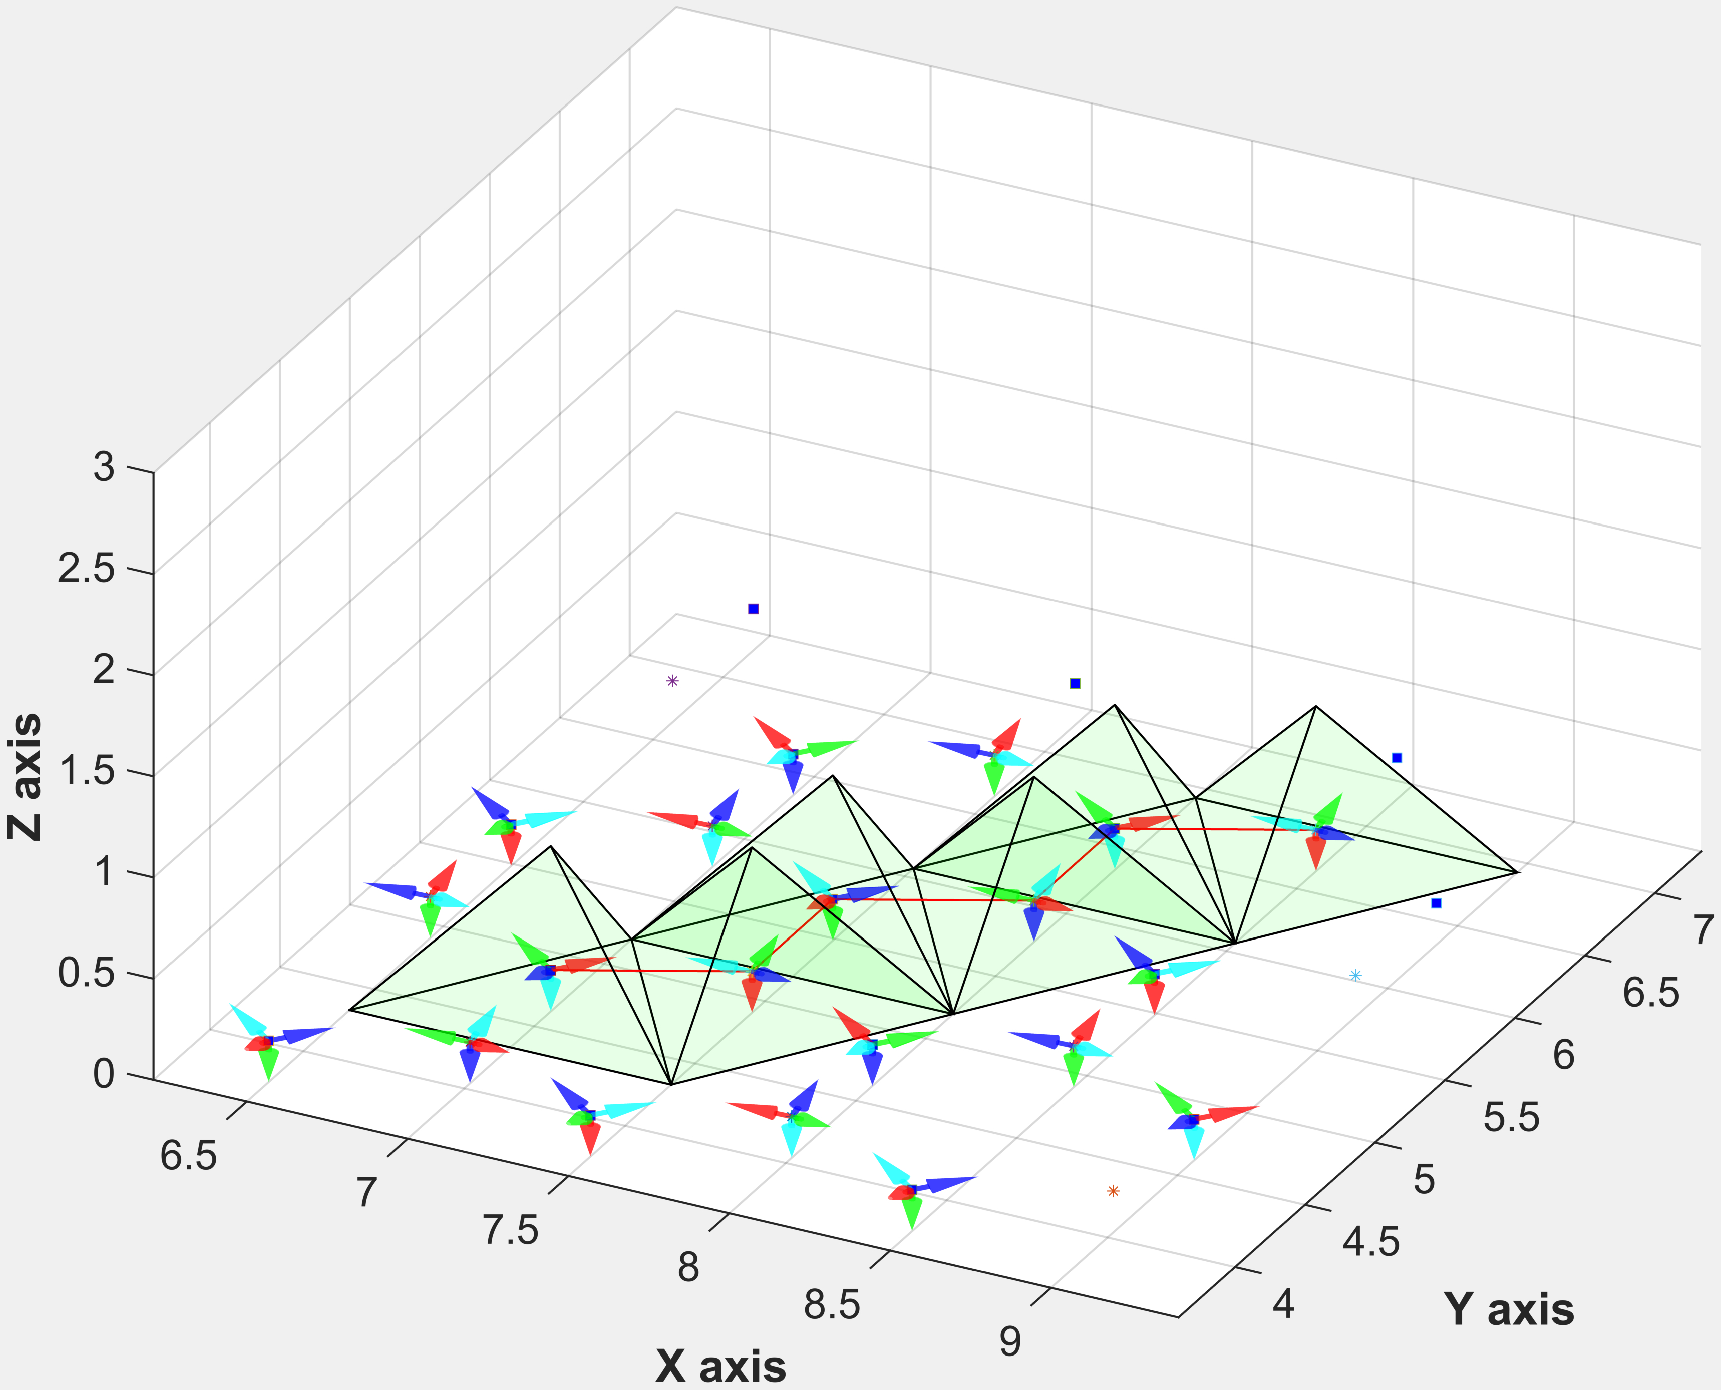
\includegraphics[page=1,width=.5\textwidth]{image/Tetra1.pdf}
	\label{fig:Tetra1Case1}
	}
\hfill
\subfigure[First four paths of the cube rolling]{
	\includegraphics[width=0.5\textwidth]{image/test3.png}
	\label{fig:Tetra2Case1}
	}
\caption{Blah Blah Tetra2}
\end{figure}
\end{center}

%%
%%
%%
%%
\noindent\uline{Case study 3}: Bi-direction path finding.\\
%%
%%
%%

\noindent\uline{Case study 4}: Cube path planning with obstacle avoiding.\\
%%
%%
%%

\noindent\uline{\textbf{Octahedron solid}}:
Dennis also went his own way and divided the sides of the triangles into equal-angles (as measured from the center of the geodesic), instead of equal-length pieces. This technique is slightly more effective at evenly distributing the triangles across the surface of the sphere. For example, compare an octahedron subdivided with frequency 20, using the linear technique (as outlined by the quiz) versus the angular technique Dennis used in this picture. Note how the linear technique has the triangles piling up along the edges of the original face of the octahedron, where the radial technique does a better job of spacing them out.\\

\begin{center}
\begin{figure}[h]
\subfigure[The initial configuration is the same position but different orientation with goal configuration]{
	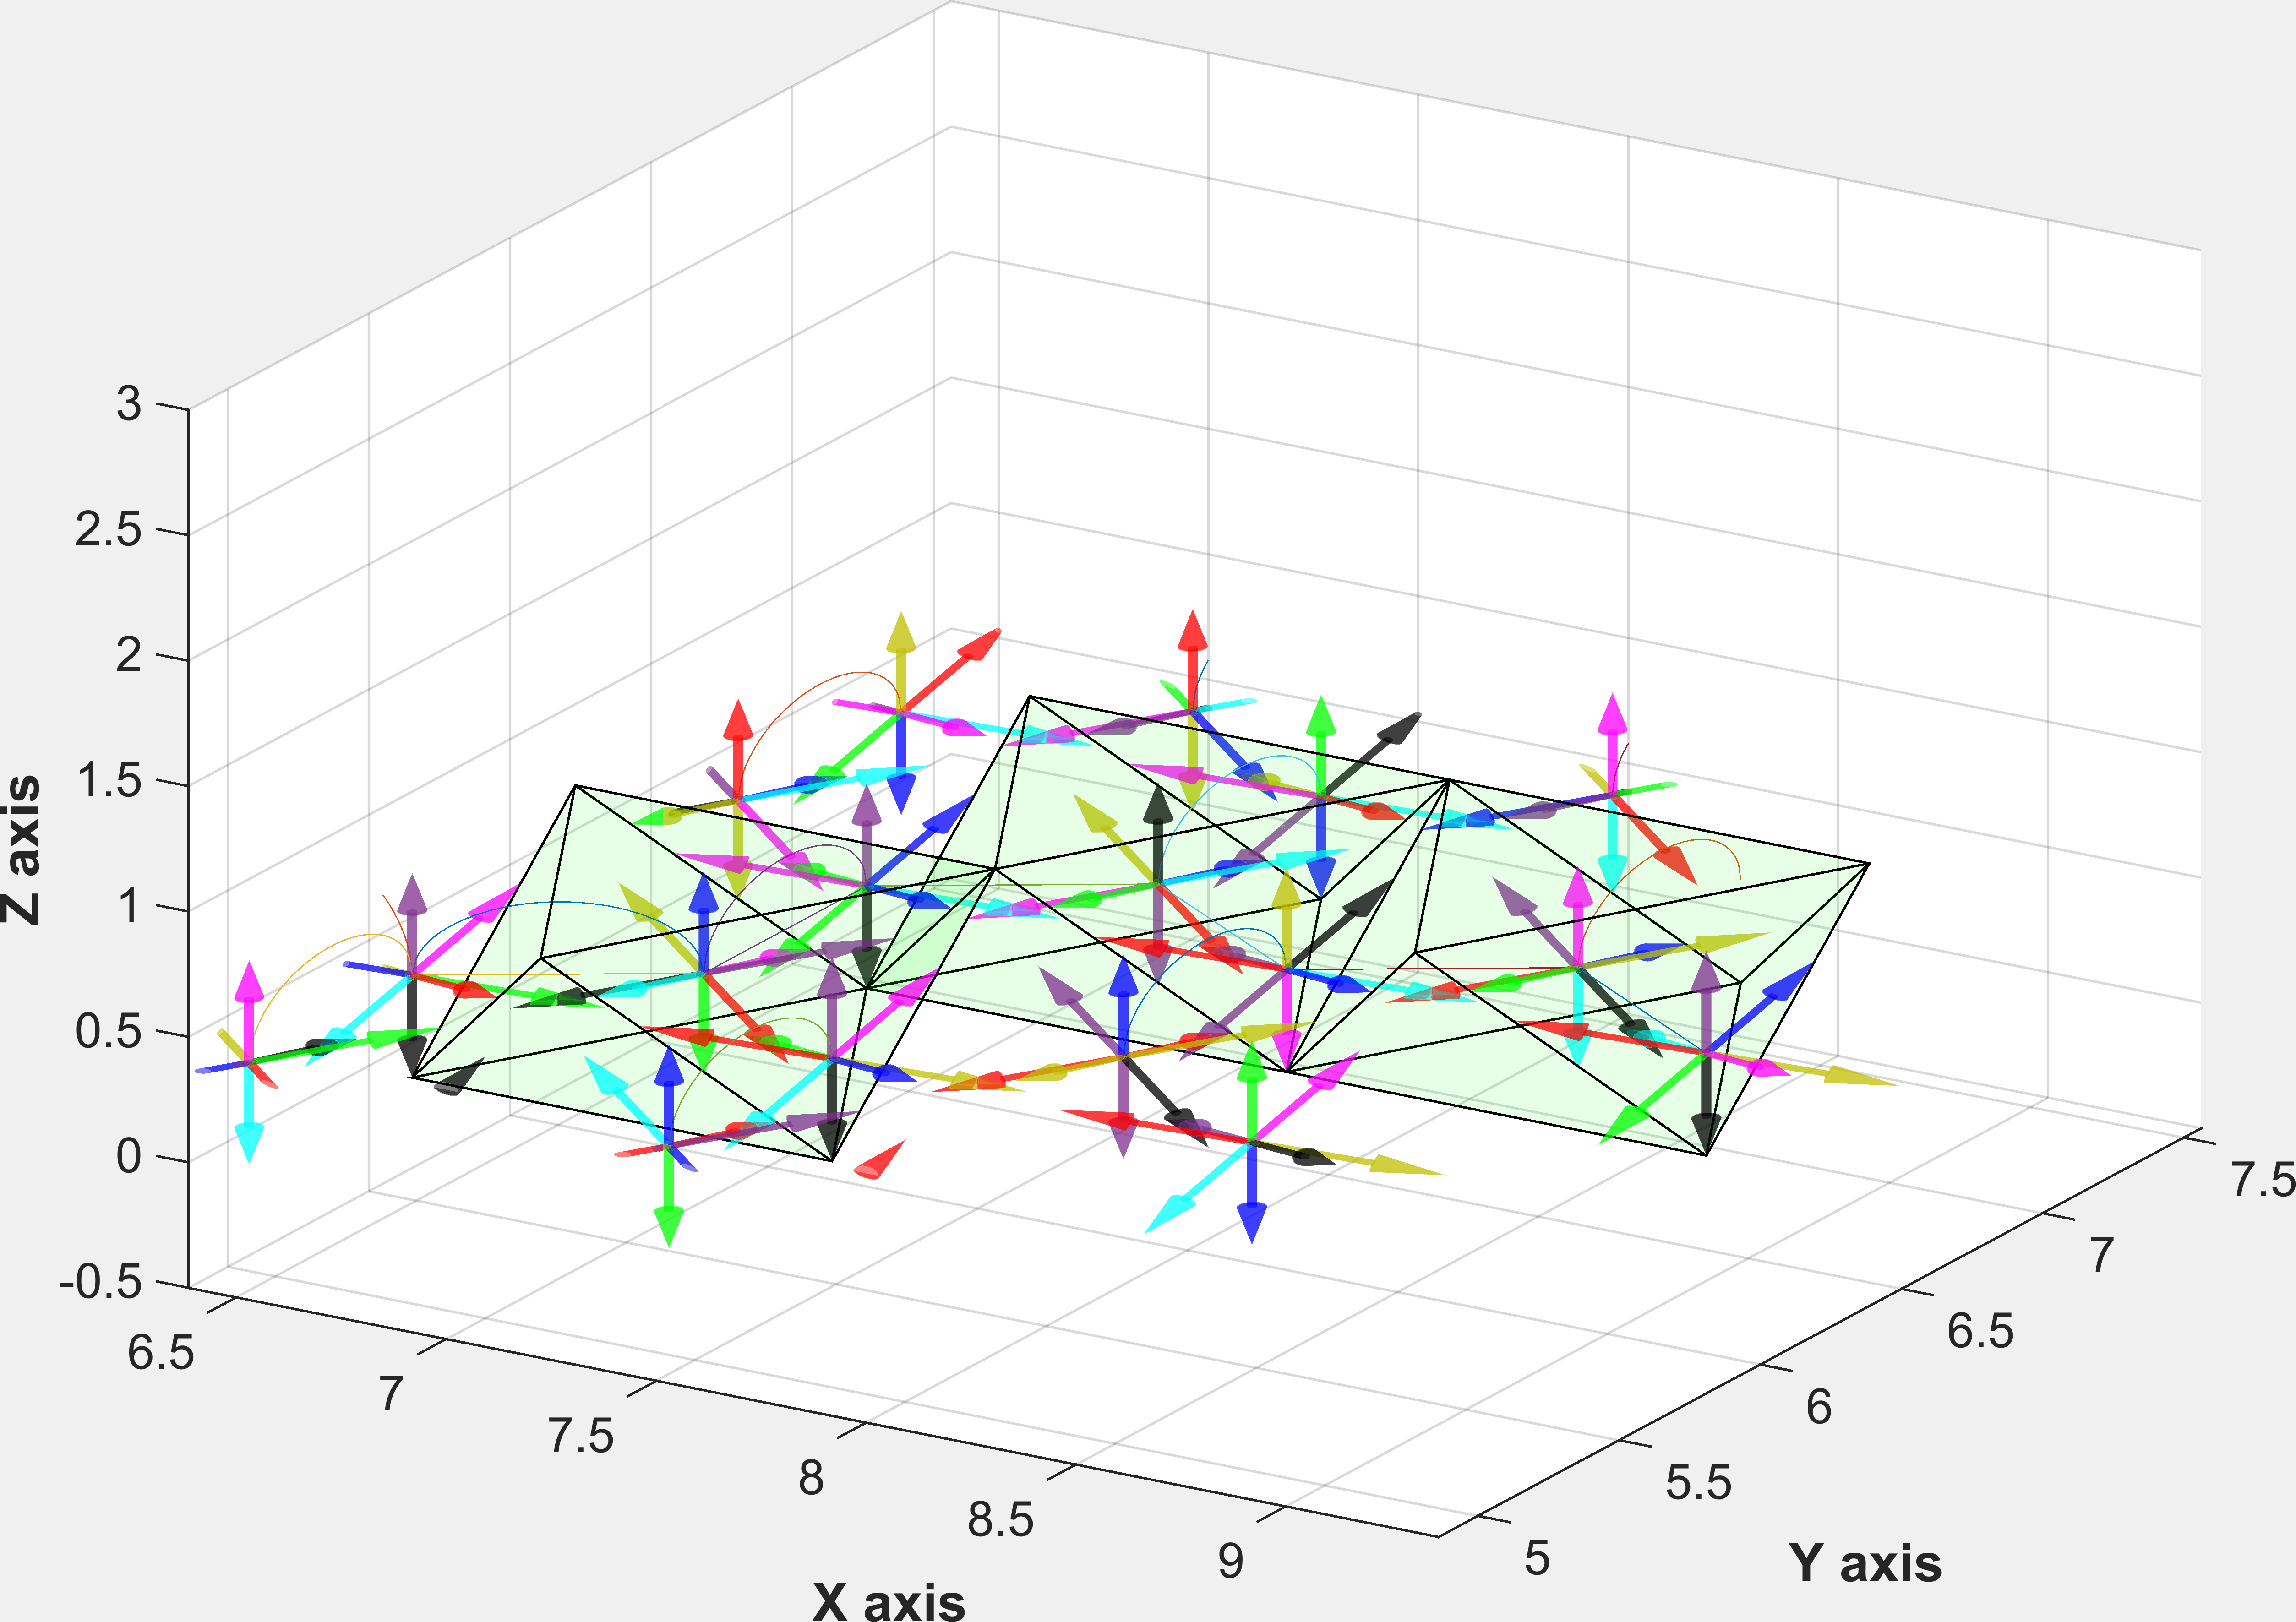
\includegraphics[width=0.5\textwidth]{image/Octa1.png}
	\label{fig:Octa1Case1}
	}
\hfill
\subfigure[First four paths of the cube rolling]{
	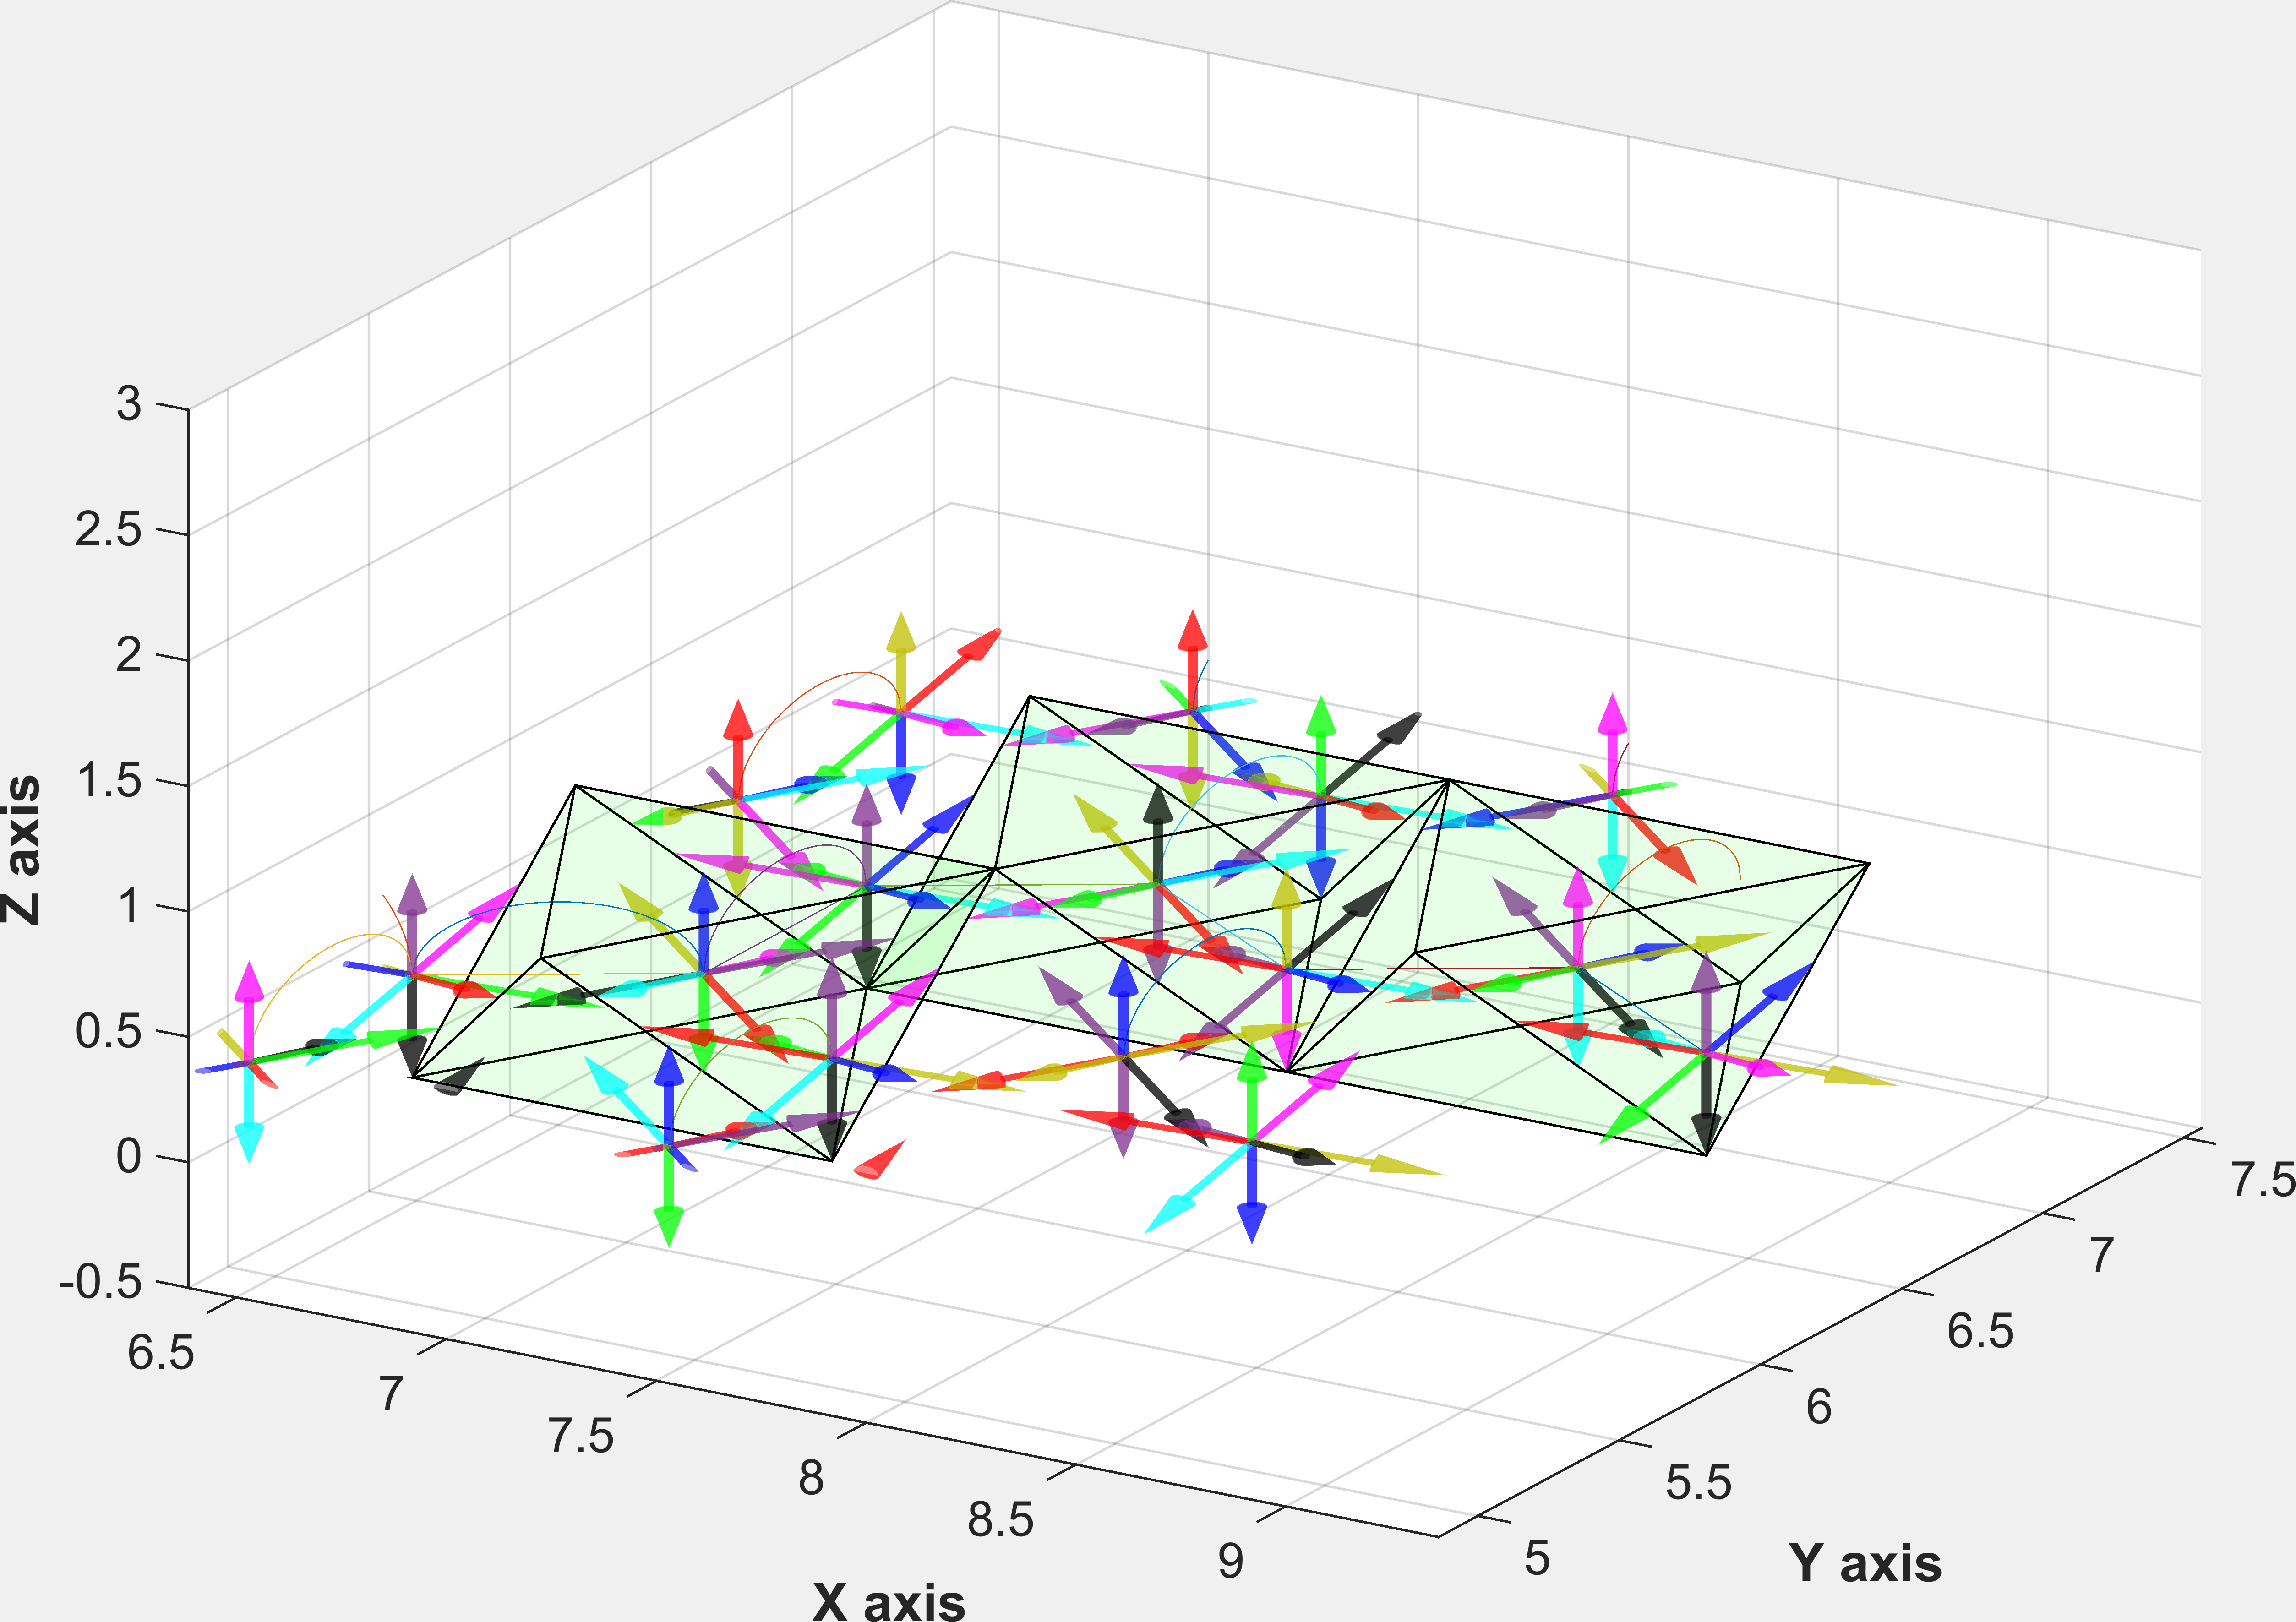
\includegraphics[width=0.5\textwidth]{image/Octa1.png}
	\label{fig:Octa1Case1}
	}
\caption{Blah Blah Octa}
\end{figure}
\end{center}

\noindent\uline{\textbf{Icosahedron solid}}:
Writing about cube solid properties\\

\noindent\uline{\textbf{Dodecahedron}}:
Writing about cube solid properties\\


\noindent\uline{\textbf{Experiments}}:
Writing about cube solid properties\\

\noindent\uline{\textbf{Discussion}}: 
\textcolor{blue}{Q2 \& Q3\\
- Q2: What are the new things you learned after you did whatever you did?\\
- Q3: What exactly did you do?}\\

\begin{itemize}
\color{red}
\item \textbf{Discussion}
\item \textit{What your results mean}
\item \textit{Why it makes a difference}
\item \textbf{Conclusion}
\item \textit{Broader implications}
\item \textit{Areas for further study}
\end{itemize}





